%!TEX root = main.tex
\section{Results}

The Dieleman model was used for both sex and speaker classification. The results are presented below.

\begin{table}[H]
\centering
\begin{tabular}{r|c|c}
model & TIMIT & ELSDSR \\ \hline
                    Baseline & $0.354$ & $0.465$ \\
                    Logistic & $0.094 \pm 0.012$ & $0.030 \pm 0.007$ \\
                 GMM on MFCC & $0.192 \pm 0.024$ & $0.140 \pm 0.019$ \\
                    Dieleman & $0.093 \pm 0.012$ & $0.026 \pm 0.006$ \\
     Dieleman + L2 & $0.114 \pm 0.013$ & $0.036 \pm 0.016$ \\
  Dieleman + Scale & $0.111 \pm 0.015$ & $0.022 \pm 0.006$ \\
 Dieleman + Offset & $0.107 \pm 0.008$ & $0.027 \pm 0.014$ \\
\end{tabular}
\caption{misclassification rate for sex classification with $95\%$ confidence interval.}
\label{tab:results-sex}
\end{table}

\begin{table}[H]
\centering
\begin{tabular}{r|c|c}
model & TIMIT & ELSDSR \\ \hline
                    Baseline & $0.988$ & $0.957$ \\
                    Logistic & $0.796 \pm 0.046$ & $0.338 \pm 0.043$ \\
                 GMM on MFCC & $0.836 \pm 0.020$ & $0.391 \pm 0.023$ \\
                    Dieleman & $0.965 \pm 0.021$ & $0.570 \pm 0.029$ \\
     Dieleman + L2 & $0.944 \pm 0.020$ & $0.552 \pm 0.045$ \\
  Dieleman + Scale & $0.973 \pm 0.007$ & $0.640 \pm 0.110$ \\
 Dieleman + Offset & $0.971 \pm 0.006$ & $0.628 \pm 0.117$ \\
\end{tabular}
\caption{misclassification rate for speaker classification with $95\%$ confidence interval.}
\label{tab:results-speaker}
\end{table}

As seen the Dieleman model does not appear to be better than a simple logistic model or the GMM. Because the logistic model can be expressed as a simple neural network, we attempted to expand the logistic network with individual layers form the Dieleman network, however all configuration that uses convolutional layers performed similarly to the Dieleman network.

The regularization parameter for Weight Decay (L2) in the speaker classification was optimized. Similar procedure could have been done on the Scale Invariant and Offset Invariant regularizers, however the implementation of those where so slow that we considered it infeasible for the Dieleman network.

\begin{figure}[H]
  \centering
  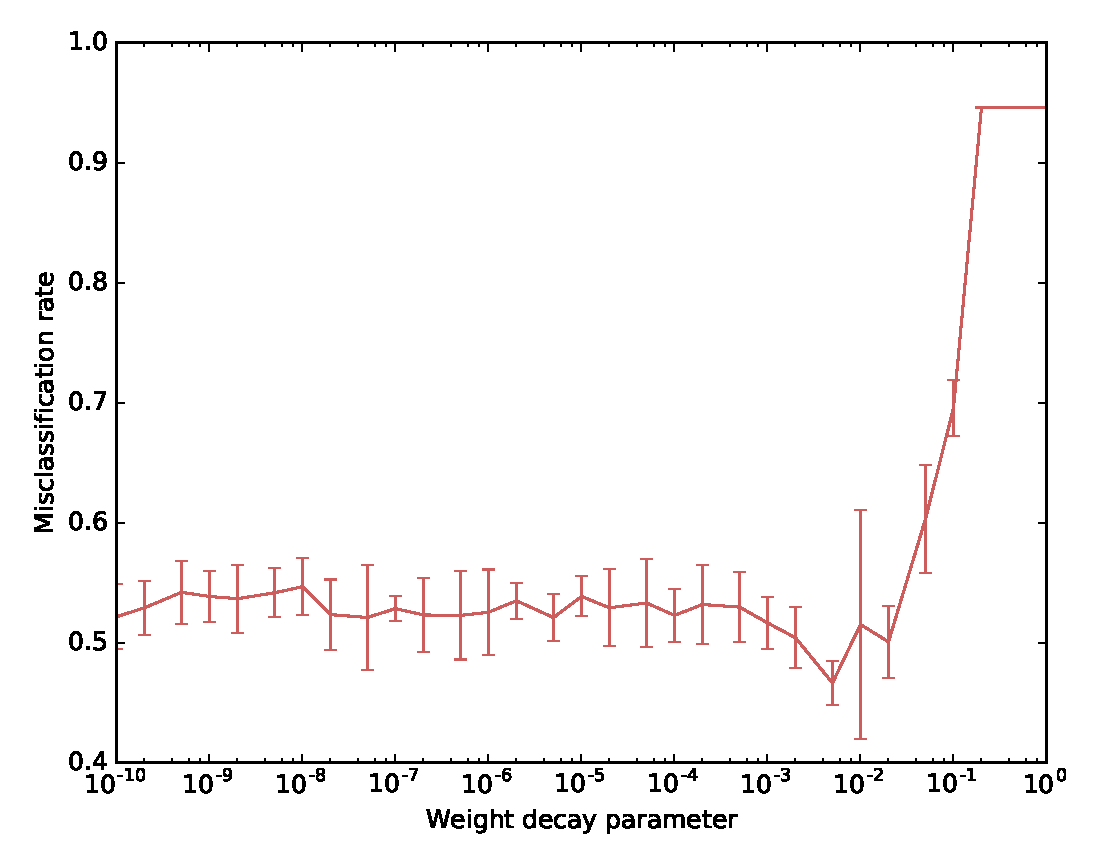
\includegraphics[width=0.4\textwidth]{plots/reg_opt_dieleman_speaker_elsdsr}
  \caption{Weight decay optimization for the speaker classification problem on the ELSDSR dataset, using $5$-fold cross-validation.}
  \label{fig:reg_opt}
\end{figure}

The best regularizer parameter is $\lambda = 5 \cdot 10^{-3}$, to ensure it is statistically significantly different from choosing $\lambda = 0$ a two-sample t-test was used. This yields $p = 0.00070$, i.e. it is significant with $95\%$ confidence.

\subsection{Analysis on generated datasets}

Because the Scale Invariant and Offset Invariant regularizers did not improve the results on sex or speaker classification, the regularizers was analyzed using generated dimensional datasets.

\todo[inline]{elaborate on the generated datasets}

For each dataset generator the optimal regularization parameters where chosen. This was done by sampling 10 datasets for each data generator, model and regularization choice. The results can be seen in \cref{appendix:regualization-optimization}. The best parameters was then used to compare the models, see \cref{fig:2d_significant}.

\begin{figure}[h]
	\centering
	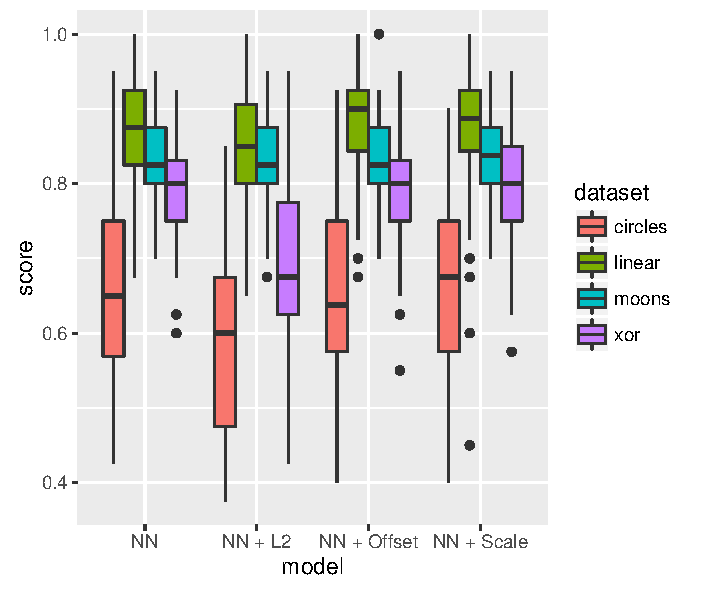
\includegraphics[width=0.45\textwidth]{plots/2d_significant}
	\caption{Boxplot of misclassification rate over 100 datasets.}
	\label{fig:2d_significant}
\end{figure}

As seen from \cref{fig:2d_significant} is no significant benefit of using any of the regularizers. However misclassification only tests the decision boundary, thus it made sense to inspect the probability function contours, also here no difference could be observed (see \cref{appendix:generated-contour-optimized}). Finally the regularizers where checked for extreme regularization parameter choices \cref{plt:generated-contour-extream}.

\begin{figure*}[ht]
	\centering
	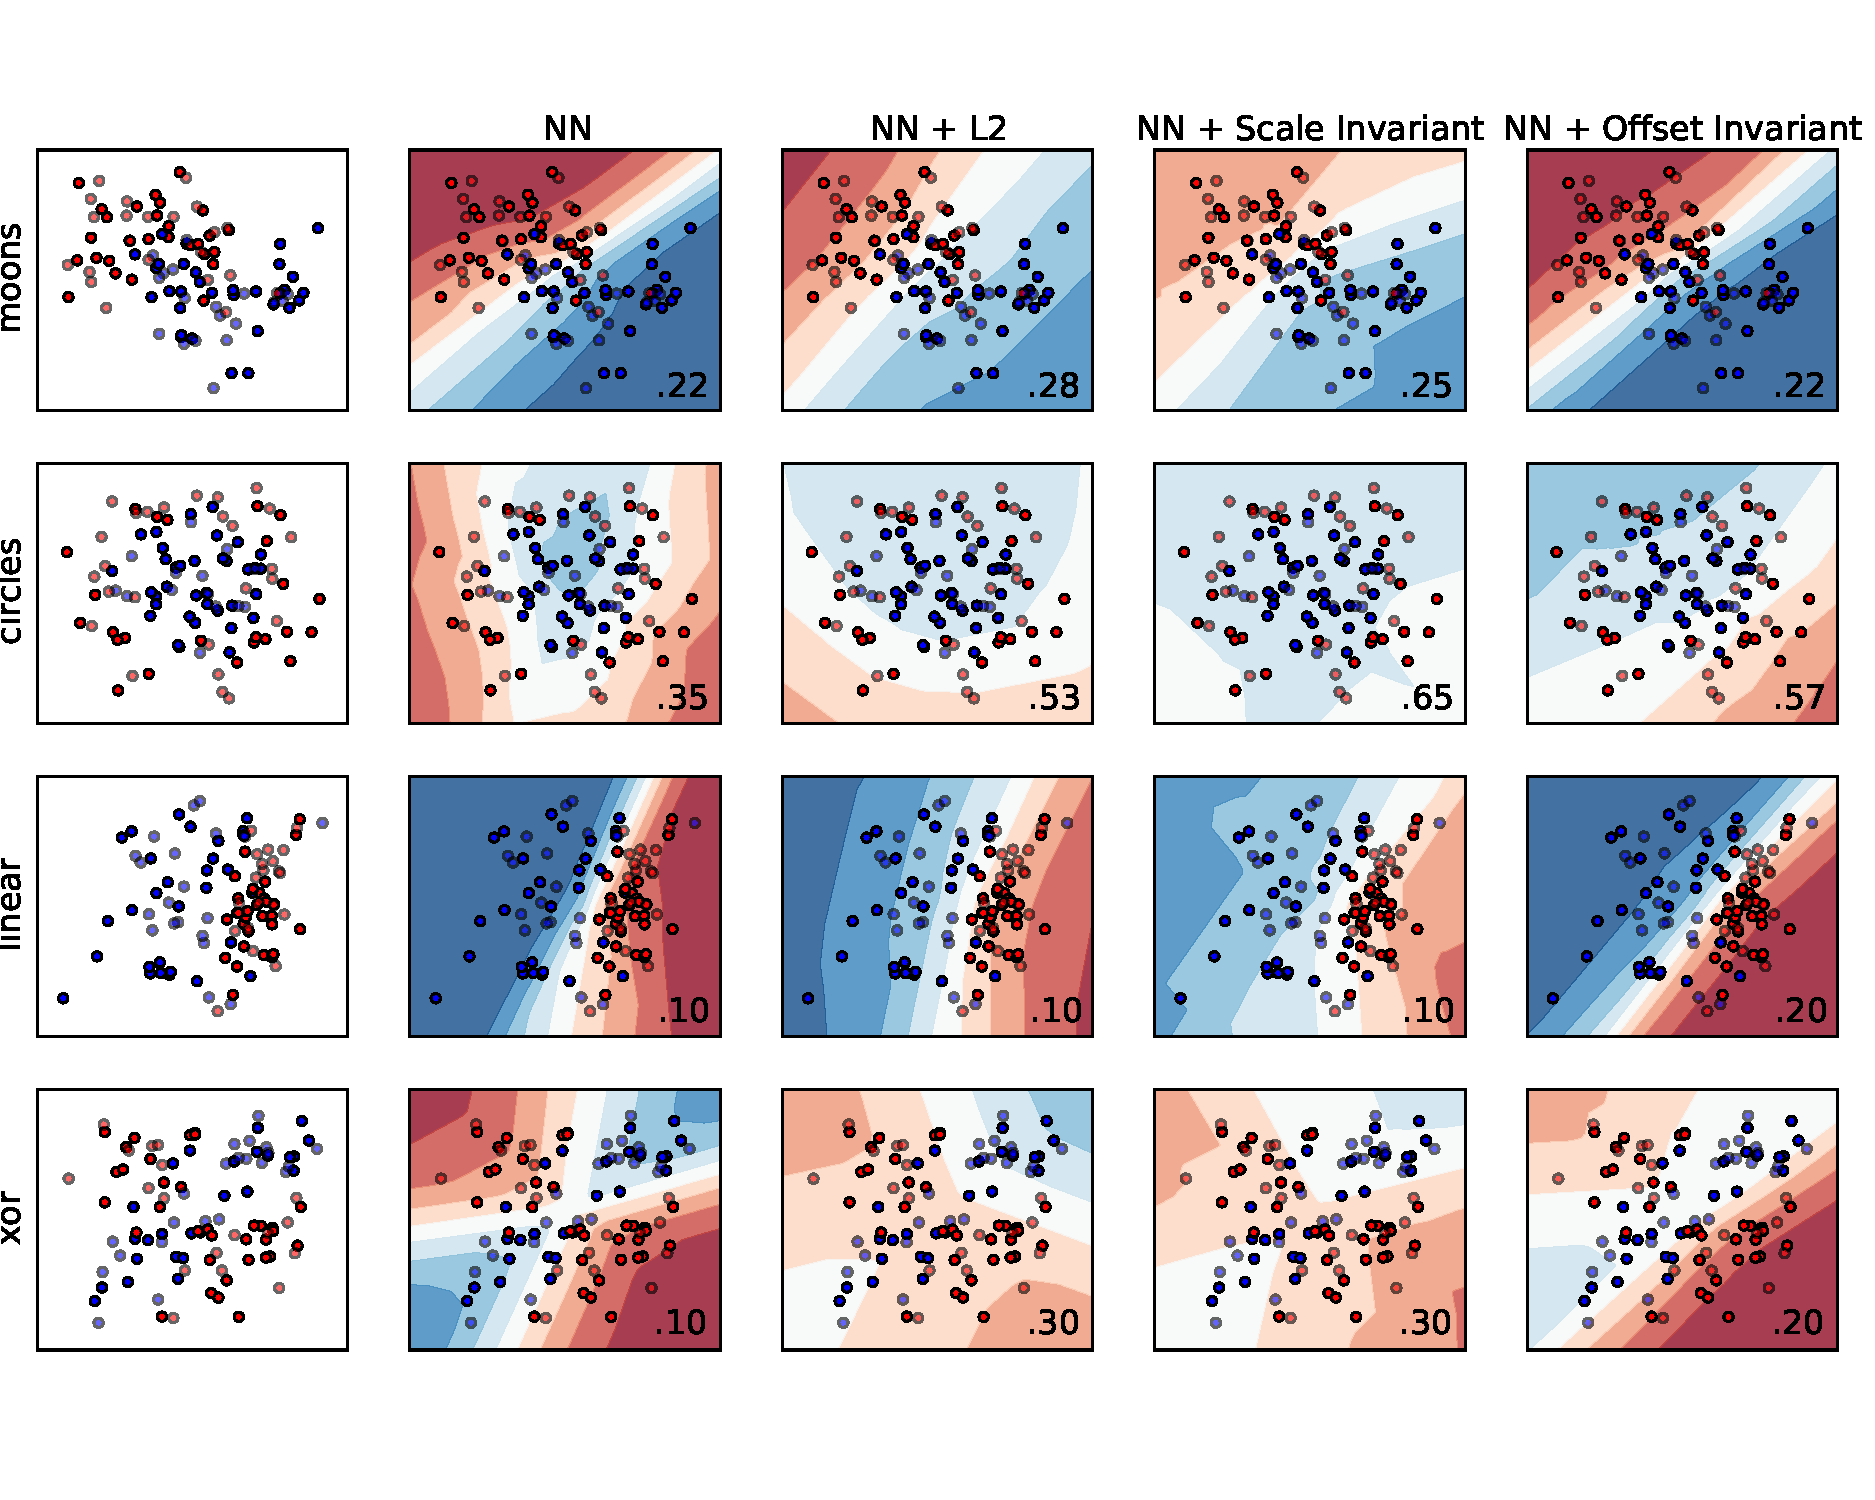
\includegraphics[width=0.7\textwidth, trim = 0 2.2cm 0 1.5cm, clip]{plots/2d_classifier-extream}
	\caption{Observations and contour plot of the class probability function for each classifier and dataset. The regularizer parameters was set to extreme values such the effect is visible. $0.1$ for \textit{NN + L2} and $10$ for \textit{NN + Scale/Offset Invariant}.}
	\label{plt:generated-contour-extream}
\end{figure*}

